%%%%%%%%%%%%%%%%%%%%%%%%%%%%%%%%%%%%%%%%%
% Make sure to set your name, legi number and url to the right git branch.
\newcommand{\hmwkAuthorName}{Marc Fischer} % Your name
\newcommand{\hmwkAuthorLegi}{13-943-568} % Your name
\newcommand{\hmwkGitBranch}{13-943-568/1\_locally\_linear\_embedding} % Your name
%
%%%%%%%%%%%%%%%%%%%%%%%%%%%%%%%%%%%%%%%%%

%----------------------------------------------------------------------------------------
%	PACKAGES AND OTHER DOCUMENT CONFIGURATIONS
%	Skip this
%----------------------------------------------------------------------------------------

\documentclass{article}

\usepackage{fancyhdr} % Required for custom headers
\usepackage{lastpage} % Required to determine the last page for the footer
\usepackage{extramarks} % Required for headers and footers
\usepackage{graphicx} % Required to insert images
\usepackage{lipsum} % Used for inserting dummy 'Lorem ipsum' text into the template


% Margins
\topmargin=-0.45in
\evensidemargin=0in
\oddsidemargin=0in
\textwidth=6.5in
\textheight=9.0in
\headsep=0.25in 

\linespread{1.1} % Line spacing

% Set up the header and footer
\pagestyle{fancy}
\lhead{\hmwkAuthorName} % Top left header
\chead{\hmwkClass\ \hmwkTitle} % Top center header
\rhead{\firstxmark} % Top right header
\lfoot{\lastxmark} % Bottom left footer
\cfoot{} % Bottom center footer
\rfoot{Page\ \thepage\ of\ \pageref{LastPage}} % Bottom right footer
\renewcommand\headrulewidth{0.4pt} % Size of the header rule
\renewcommand\footrulewidth{0.4pt} % Size of the footer rule

\setlength\parindent{0pt} % Removes all indentation from paragraphs

%----------------------------------------------------------------------------------------
%	DOCUMENT STRUCTURE COMMANDS
%	Skip this
%----------------------------------------------------------------------------------------

% Header and footer for when a page split occurs within a problem environment
\newcommand{\enterProblemHeader}[1]{
\nobreak\extramarks{#1}{#1 continued on next page\ldots}\nobreak
\nobreak\extramarks{#1 (continued)}{#1 continued on next page\ldots}\nobreak
}

% Header and footer for when a page split occurs between problem environments
\newcommand{\exitProblemHeader}[1]{
\nobreak\extramarks{#1 (continued)}{#1 continued on next page\ldots}\nobreak
\nobreak\extramarks{#1}{}\nobreak
}

\setcounter{secnumdepth}{0} % Removes default section numbers
\newcounter{homeworkProblemCounter} % Creates a counter to keep track of the number of problems

\newcommand{\homeworkProblemName}{}
\newenvironment{homeworkProblem}[1][Problem \arabic{homeworkProblemCounter}]{ % Makes a new environment called homeworkProblem which takes 1 argument (custom name) but the default is "Problem #"
\stepcounter{homeworkProblemCounter} % Increase counter for number of problems
\renewcommand{\homeworkProblemName}{#1} % Assign \homeworkProblemName the name of the problem
\section{\homeworkProblemName} % Make a section in the document with the custom problem count
\enterProblemHeader{\homeworkProblemName} % Header and footer within the environment
}{
\exitProblemHeader{\homeworkProblemName} % Header and footer after the environment
}

\newcommand{\problemAnswer}[1]{ % Defines the problem answer command with the content as the only argument
\noindent\framebox[\columnwidth][c]{\begin{minipage}{0.98\columnwidth}#1\end{minipage}} % Makes the box around the problem answer and puts the content inside
}

\newcommand{\homeworkSectionName}{}
\newenvironment{homeworkSection}[1]{ % New environment for sections within homework problems, takes 1 argument - the name of the section
\renewcommand{\homeworkSectionName}{#1} % Assign \homeworkSectionName to the name of the section from the environment argument
\subsection{\homeworkSectionName} % Make a subsection with the custom name of the subsection
\enterProblemHeader{\homeworkProblemName\ [\homeworkSectionName]} % Header and footer within the environment
}{
\enterProblemHeader{\homeworkProblemName} % Header and footer after the environment
}
   
%----------------------------------------------------------------------------------------
%	NAME AND CLASS SECTION
%	Skip this
%----------------------------------------------------------------------------------------

\newcommand{\hmwkTitle}{Locally Linear Embedding} % Assignment title
\newcommand{\hmwkDueDate}{Monday,\ March\ 6th,\ 2017} % Due date
\newcommand{\hmwkClass}{SLT coding exercise\ \#1} % Course/class
\newcommand{\hmwkClassTime}{Mo 16:15} % Class/lecture time
\newcommand{\hmwkClassInstructor}{} % Teacher/lecturer

%----------------------------------------------------------------------------------------
%	TITLE PAGE
%	Skip this
%----------------------------------------------------------------------------------------

\title{
\vspace{2in}
\textmd{\small{\hmwkClass}}\\
\textmd{\textbf{\hmwkTitle}}\\
\small{https://gitlab.vis.ethz.ch/vwegmayr/slt-coding-exercises}\\
\normalsize\vspace{0.1in}\small{Due\ on\ \hmwkDueDate}
%\vspace{0.1in}\large{\textit{\hmwkClassInstructor\ \hmwkClassTime}}
\vspace{3in}
}

\author{
\hmwkAuthorName\\
\hmwkAuthorLegi
}

\date{ } % Insert date here if you want it to appear below your name


%----------------------------------------------------------------------------------------
%	MY OWN HEADER SECTION
%----------------------------------------------------------------------------------------


\usepackage{amsmath,amssymb} % math
\usepackage{graphicx,subcaption,float,wrapfig} %figures and graphics
\usepackage[font={small,it}]{caption}
\usepackage{listings}
\usepackage{hyperref}
\DeclareMathOperator*{\argmin}{arg\,min} %argmin operator

\graphicspath{{images/}}

\begin{document}

\maketitle

%----------------------------------------------------------------------------------------
%	TABLE OF CONTENTS
%	Skip this
%----------------------------------------------------------------------------------------

%\setcounter{tocdepth}{1} % Uncomment this line if you don't want subsections listed in the ToC

\newpage
\tableofcontents
\newpage

%----------------------------------------------------------------------------------------
%	SECTIONS
%	Now you are in the right hood
%----------------------------------------------------------------------------------------

\begin{homeworkProblem}[The Model]
\vspace{10pt}

\textbf{Input}
\begin{itemize}
	\item data $\mathbf{X} = \{\mathbf{x}_1, \dots, \mathbf{x}_N \}, \quad \mathbf{x}_i \in \mathbb{R}^D$
	\item target dimension $d$
	\item some distance metric, along with integer $K$ or radius $r$, which determines the size of the neighborhood
\end{itemize}

\textbf{Output}
\begin{itemize}
	\item $Y = \{ \mathbf{y}_i \}$ such that $\mathbf{x}_i$ is a $d$-Dimensional representation of $x_i$
\end{itemize}

\textbf{Algorithm and equations}
Given high dimensional data $\mathbf{X} = \{\mathbf{x}_1, \dots, \mathbf{x}_N \}, \quad \mathbf{x}_i \in \mathbb{R}^D$, we want to represent it in a low dimensional space $\mathbb{R}^d$, $d \ll D$. The Local Linear Embedding algorithm accomplishes this in 3 steps.

\begin{enumerate}
	\item For each $\mathbf{x}_i$ compute the neighborhood $N(\mathbf{X}_i)$. Either find the $K$ nearest $\mathbf{x}_j$ or consider a fixed radius around $\mathbf{x}_i$. We will denote the neighborhood of $\mathbf{x}_i$ by $\mathcal{N}(\mathbf{x})_i$. And define it as

	\begin{align} \label{eq:neighborhood}
		\mathcal{N}(\mathbf{x}_i) = \argmin_{\substack{j_1, \dots, j_k\\\forall k \in [1,K] j_k \neq i\\\forall k<l \in [1,K] j_k \neq j_l }} \sum_{j_1, \dots, j_k} \| \mathbf{x}_i - \mathbf{x}_{j_k} \|.
	\end{align}
	Other distance metrics can be used. I will investigate mutal information as such.
	


	\item Find weights $\mathbf{W}$ such that the error in equation~\ref{eq:weightError}  is minimal. For a point $\mathbf{x}_i$ the weights $w_{ij}$ describe how the vector $\mathbf{x}_i$ can be reconstructed from other vectors. For a certain $j$ the weight $w_{ij}$ indicates how much $\mathbf{x}_j$ contributes to this reconstruction. We also require that only for $j \in \mathcal{N}(\mathbf{x}_i)$ the weight $w_{ij}$ is non-zero and that $\sum_j w_{ij} = 1$

	\begin{align} \label{eq:weightError}
		\mathcal{E}(\mathbf{W}) = \sum_i \| \mathbf{x}_i - \sum_j w_{ij} \mathbf{x}_j \|^2	
	\end{align}.

	\item Compute the vectors $\mathbf{y}_i$ such that the following error term is minimized. The resulting $\mathbf{y}_i$ is a $d$-dimensional description of $\mathbf{x}_i$.

	\begin{align} \label{eq:embeddingError}
		\mathcal{E}(\mathbf{y}_1, \dots, \mathbf{y}_N) = \sum_i \| \mathbf{y}_i - \sum_j w_{ij} \mathbf{y}_j \|^2
	\end{align}


\end{enumerate}

\end{homeworkProblem}
\clearpage

%----------------------------------------------------------------------------------------
\begin{homeworkProblem}[The Questions]
For the ease of writing I created my own section structure. In the parenthesis after the section name I indicate which of the original subproblems I address.

\begin{homeworkSection}{LLE and Neighborhood (a, b, d)}
\begin{wrapfigure}[16]{R}{0.35\textwidth}
	\vspace{-50pt}
    \centering
    \begin{subfigure}[b]{0.35\textwidth}
    	\resizebox{\linewidth}{!}{
    	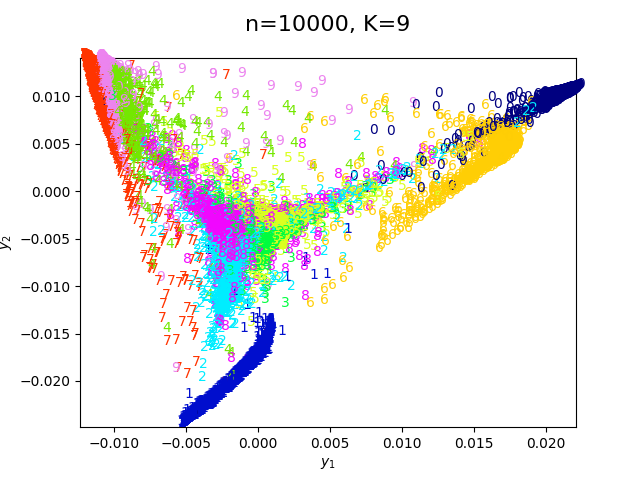
\includegraphics{2d_10000_9.png}}
    \end{subfigure}
    \\
    \begin{subfigure}[b]{0.35\textwidth}
    	\resizebox{\linewidth}{!}{
    	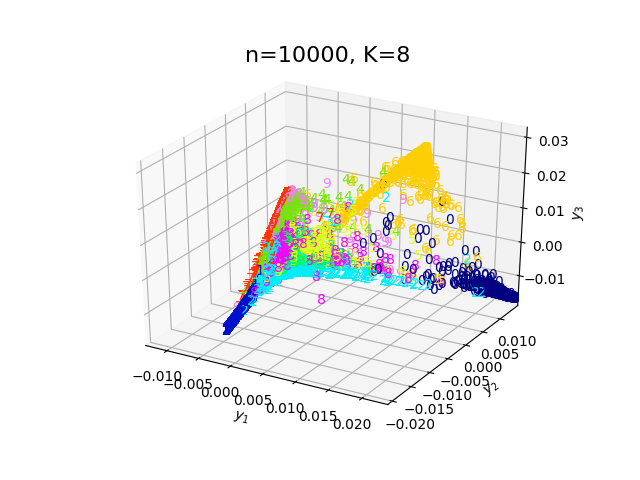
\includegraphics{3d_10000_8.png}}
    \end{subfigure}
    \caption{Visualizations of LLE in 2D and 3D for best $K$.}
    \label{fig:plotBestK}
\end{wrapfigure}

Figure~\ref{fig:plotBestK} shows the clustering in 2D and 3D respectively. We can clearly see clusters for the different numbers. The best $K$ (size of neighborhood) for 2D seems to be around 9 and for 3D around 8.

\subsubsection{Effects of different K (d)}

For higher $K$ first there forms a cluster of 1s and a cluster of all other numbers. For even higher $K$ they all merge into one cluster. The effect of the ones separating is likely due to the fact that they are the most different class to all others.
The merging into one cluster for high $K$ is probably due to the fact that the large neighborhoods often include numbers from different categories. Thus we need to describe most with few linear models.
For lower $K$ the numbers again lump into a single cluster. Probably because there weights carry too little information, to really form clusters.
The effects of high and low K can be seen in Figure~\ref{fig:plotBadK} on page \pageref{fig:plotBadK}.

\subsubsection{Mutual information as similarity measure}

A quick search of literature and Google suggested that a common similarity metric for images is their mutual information. The probabilities for the mutual information are estimated by histograms. I also implemented LLE where there the K nearest neighbors with highest mutual information are used to form the neighborhood. Figure~\ref{fig:mi_neighborhood} visualizes the neighborhood defined by the mutual information.

\begin{wrapfigure}[19]{R}{0.35\textwidth}
	\vspace{-20pt}
	\centering
	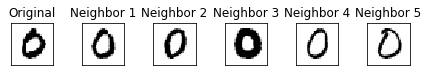
\includegraphics[width=0.35\textwidth]{mi_neighborhood.png}
    \caption{The $K = 5$ neighborhood of the image on the left, as measured by mutual information.}
    \label{fig:mi_neighborhood}
\end{wrapfigure}

Figure~\ref{fig:plotMI} shows the resulting LLEs. Again we see that for low $K$ (around 4-5) we have somewhat well separated clusters. Results for higher $K$ again merge into one big cluster. However around $K = 40$ they start to get better again (see Figure~\ref{fig:plotMI40} on page \pageref{fig:plotMI40}).
It should be noted that the computation of the mutual information is much more expensive than the the euclidean distances (which is why I show $n=1000$ instead of $n=10000$).

\end{homeworkSection}

\begin{homeworkSection}{Cluster structure (c)}

\begin{wrapfigure}[10]{r}{0.55\textwidth}
	\vspace{-30pt}
    \centering

    \begin{subfigure}[b]{0.245\textwidth}
    	\resizebox{\linewidth}{!}{
    	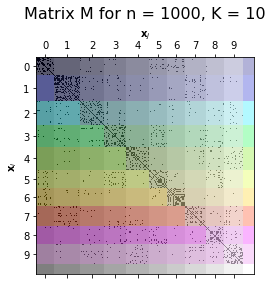
\includegraphics{M_1000.png}}
	    \caption{Structure of matrix M.}
	    \label{fig:M}
    \end{subfigure}
	~
    \begin{subfigure}[b]{0.245\textwidth}
    	\resizebox{\linewidth}{!}{
    	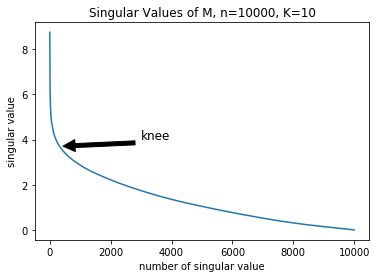
\includegraphics{singular_values_M.png}}
    \caption{Singular values of the matrix M.}
    \label{fig:singular_values_M}
    \end{subfigure}
    \caption{Investigation of matrix M.}
    \label{fig:Mdetails}
\end{wrapfigure}

Figure~\ref{fig:M} shows the structure of Matrix M, when the rows and columns are rearranged with respect to their class.
We clearly see that there are diagonal blocks representing the clusters, but also a lot of off-diagonal noise. Those are just random interaction between the clusters, but we can also observe that they increase between similar looking numbers such as 0 and 6. For larger $n$ these trends get harder to spot as clusters become smaller relative to the whole matrix. This can be seen in Figure~\ref{fig:M10k} on page \pageref{fig:M10k}.
Figure~\ref{fig:singular_values_M} shows the singular values of the matrix M. We see a knee in the plot. Left of the knee eigenvalues are much larger than those to the right. An ideal dimension would be somewhere in that knee. This is similar to what one does in PCA.

\end{homeworkSection}

\begin{figure}[H]
    \centering
    \begin{subfigure}[b]{0.45\textwidth}
    	\resizebox{\linewidth}{!}{
    	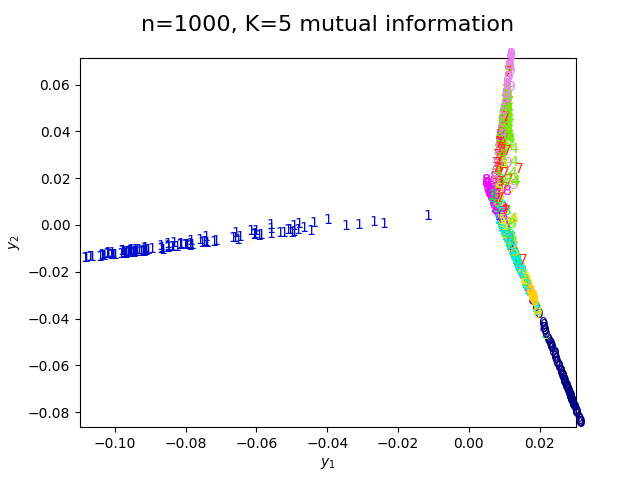
\includegraphics{mi_2d_1000_5.png}}
    \end{subfigure}
    ~
    \begin{subfigure}[b]{0.45\textwidth}
    	\resizebox{\linewidth}{!}{
    	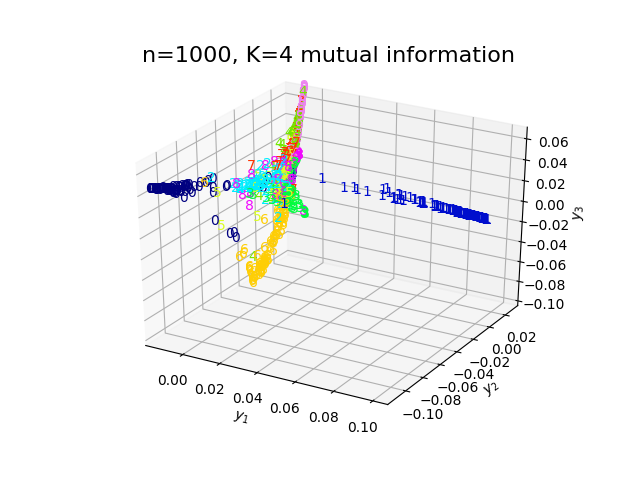
\includegraphics{mi_3d_1000_4.png}}
    \end{subfigure}
    \caption{Visualizations of LLE in 2D and 3D using mutual information to measure similarity.}
    \label{fig:plotMI}
\end{figure}

\begin{homeworkSection}{Linear manifold interpolation (e)}
\begin{wrapfigure}{r}{0.3\textwidth}
	\vspace{-20pt}
    \centering
    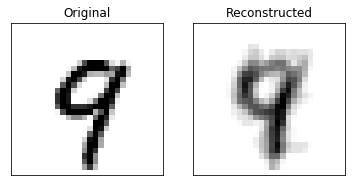
\includegraphics[width=0.3\textwidth]{reconstructed.png}
    \caption{Reconstruction of a number.}
    \label{fig:reconstruction}
\end{wrapfigure}

In order to map a point $\mathbf{y_i}$ from the embedding space back to the original space one:
\begin{enumerate}
	\item finds the neighborhood $\mathcal{N}(\mathbf{y}_i)$
	\item uses this neighborhoods to compute the weights $\mathbf{W}$ analogous to the weights computed in the high dimensional space when applying LLE
	\item approximate the neighborhood in the high dimensional space $\mathcal{N}(\mathbf{x}_i) \approx \hat{\mathcal{N}}(\mathbf{x}_i) = \{\mathbf{x}_j \, | \, \mathbf{y}_j \in \mathcal{N}(\mathbf{y}_i) \}$ and use this to approximate $\mathbf{x}_i \approx \sum_{\mathbf{x}_j \in \hat{\mathcal{N}}(\mathbf{x}_i)} \mathbf{W}_{ij} \mathbf{x}_j$
\end{enumerate}

Figure~\ref{fig:reconstruct_map} features two lines. The blue lies within the manifold, the red without. The reconstruction of the blue line can be found in Figure~\ref{fig:reconstruction_inside}. The left most and right most image are the original data points. The second left and second right respectively are their reconstructions. The ones in the middle are the reconstructions of the interpolation. The reconstruction of the red line is in Figure~\ref{fig:reconstruction_outside}. Although it does not lie within the manifold, we see number like shapes. This is because the shape is determined by its closed neighbors.

\begin{figure}[H]
	\vspace{-10pt}
    \centering
    \begin{minipage}{0.45\textwidth}
        \centering
        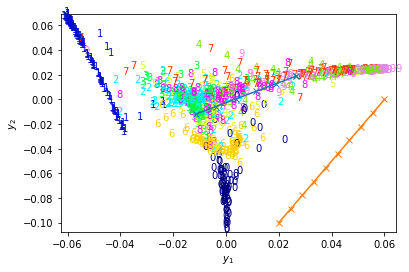
\includegraphics[width=\textwidth]{reconstruct_map.png} % first figure itself
        \caption{2D Embedding showing 2 lines. The blue within the manifold, the red without.}
        \label{fig:reconstruct_map}
    \end{minipage}\hfill
    \begin{minipage}{0.45\textwidth}
        \centering
	    \begin{subfigure}[b]{\textwidth}
	    	\resizebox{\linewidth}{!}{
	    	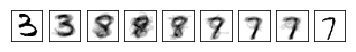
\includegraphics{reconstruct_inside_mainfold_2.png}}
	    	\caption{Reconstruction of the blue line in in Figure~\ref{fig:reconstruct_map}.}
	    	\label{fig:reconstruction_inside}
	    \end{subfigure}
	    \\
	    \begin{subfigure}[b]{\textwidth}
	    	\resizebox{\linewidth}{!}{
	    	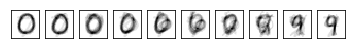
\includegraphics{reconstruct_outside_mainfold_2.png}}
	    	\caption{Reconstruction of the red line in in Figure~\ref{fig:reconstruct_map}.}
	    	\label{fig:reconstruction_outside}
	    \end{subfigure}
        \caption{Reconstructions of lines within and without the manifold.}
        \label{fig:reconstructions}
    \end{minipage}
\end{figure}


\end{homeworkSection}

\end{homeworkProblem}
\clearpage

%----------------------------------------------------------------------------------------
\begin{homeworkProblem}[The Implementation]
{
\footnotesize
\textbf{git branch}: \url{https://gitlab.vis.ethz.ch/vwegmayr/slt-coding-exercises/tree/13-943-568/1_locally_linear_embedding}\\
\textbf{implementation file}: \url{https://gitlab.vis.ethz.ch/vwegmayr/slt-coding-exercises/blob/13-943-568/1_locally_linear_embedding/lle.ipynb}
}
\vspace{-15pt}
\subsection{Nearest Neighbors}

In order to find the nearest neighbors given by Equation~\ref{eq:neighborhood} I used a fast implemenation of a KD-Tree\footnote{https://docs.scipy.org/doc/scipy-0.16.1/reference/generated/scipy.spatial.cKDTree.html}, which is a good data structure for such distance queries.

\begin{lstlisting}[language=Python, frame=single,basicstyle=\footnotesize, numbers=left]
kdt = scipy.spatial.cKDTree(data)
_,q = kdt.query(data, K+1)
\end{lstlisting}

\texttt{q[i]} then holds the indices of the $K$ nearest neighbors as well as i itself.

When I use mutual information as a similarity criterion the calculation of the nearest neighbors, based on nested loops, becomes much slower as the KD-Tree can't be used.

\subsection{Finding weights}
To find the weights, we want to minimize the error given by Equation~\ref{eq:weightError}. To do so I use the inverse local covariance matrices, as derived in exercise sheet 1 and suggested in the paper: $w_{ij} = \frac{\sum_k C^{(i)-1}_{jk} }{ \sum_{lk} C^{(i)-1}_{lk} }$.

I suspected that the inversion might be numerically problematic. It turns out that for the normal MNIST dataset this is not a problem. I had a bug in my implementation which sometimes made my $C^{(i)}_{jk}$ singular. As suggested in the original paper I added a small diagonal component to the $C^{(i)}_{jk}$ matrices. This ensures that they are not singular. After resolving the bug this was not necessary anymore, but is still in the code (see line 5 below) as it has no noticeable impact on the solution.

\begin{lstlisting}[language=Python, frame=single,basicstyle=\footnotesize, numbers=left]
W = np.zeros( (N,N) )
for i in xrange(N):
    neighborhood = q[i][1:]
    # calculate C = C^i_{jk}
    C = C + (1.0/K) * np.eye(K)
    C_inv = np.linalg.inv(C)
    noms = np.sum(C_inv, axis=1) #row wise sum
    denom = np.sum(C_inv)        
    w_ij = noms/denom
    W[i, neighborhood] = w_ij
\end{lstlisting}

\vspace{-15pt}
\subsection{Finding embedding}
To find the embedding vectors, we need to minimize Equation~\ref{eq:embeddingError}. As suggested in the paper I use the eigenvectors of $M = (\mathbb{I} - \mathbf{W})^T (\mathbb{I} - \mathbf{W})$. I started to compute them with \texttt{numpy.linalg.eig}, which worked but became very slow for larger matrices (larger numbers of data points). I switched to \texttt{scipy.linalg.eigh}, which allows to pass the range of the desired eigenvectors (i.e. the lowest $d+1$). Only computing the needed eigenvectors provided a sizable speed-up. However this computation is still the bottleneck. As mentioned in the paper a further improvement would be possible by by adapting the eigensolver so that matrix $M$ never needs to be constructed. However I decided against this, as scipy already uses high performance BLAS underneath. Creating custom code with similar performance would have required a huge time investment.

\begin{lstlisting}[language=Python, frame=single,basicstyle=\footnotesize, numbers=left]
e, v = scipy.linalg.eigh(M, eigvals=(0, d+1))
Y = v[:,1:(d+1)]
\end{lstlisting}

The current implementation runs suitably fast for $n=10000$, taking around 500s.

\end{homeworkProblem}
\clearpage

%----------------------------------------------------------------------------------------
\begin{homeworkProblem}[Your Page]

\subsection{t-SNE and PCA}
For another project in another lecture I currently use t-SNE, which also provides a very good embedding of MNIST (and high dimensional manifolds in general). Figure~\ref{fig:tsnepca} shows t-SNE on this dataset. The actual t-SNE algorithm can be applied to data of any dimension. However, usually first a PCA to some medium number of dimensions (such as 30) is applied.
I did the same for LLE. This gives a combination of two parameters to search over: The number of neighbors $K$ and the number of PCA dimensions. Below a good choice is shown. In contrast to the normal LLE we see that the cluster of ones is much tighter for example. Likely because PCA removed a lot of noise within the cluster. This is also true (to an extend) for the other clusters.\\
I firmly believe that there are still better choices for PCA-dimensions, number of neighbors and maybe the neighborhood measure.

\begin{figure}[H]
    \centering
    \begin{subfigure}[b]{0.45\textwidth}
    	\resizebox{\linewidth}{!}{
    	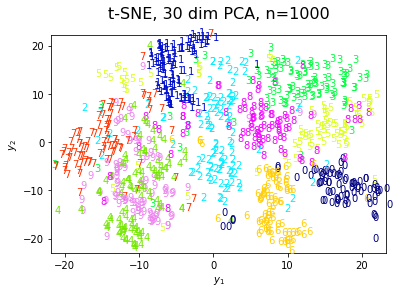
\includegraphics{t-SNE.png}}
    \end{subfigure}
    ~
    \begin{subfigure}[b]{0.45\textwidth}
    	\resizebox{\linewidth}{!}{
    	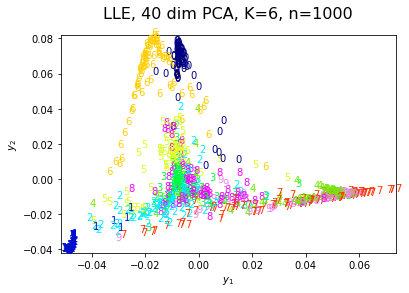
\includegraphics{LLE_PCA.png}}
    \end{subfigure}
    \caption{Visualizations of LLE and t-SNE in 2D.}
    \label{fig:tsnepca}
\end{figure}

\subsection{Appendix}
I use this section to show more plots and results that did not find into the 2 pages of the question section.

\begin{figure}[H]
    \centering
    \begin{subfigure}[b]{0.45\textwidth}
    	\resizebox{\linewidth}{!}{
    	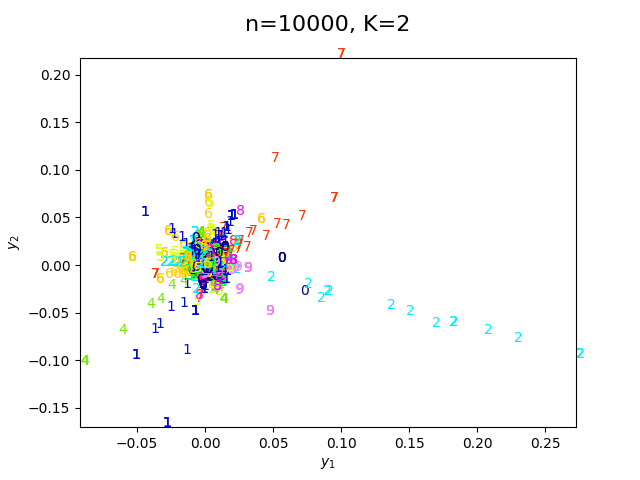
\includegraphics{2d_10000_2.png}}
    \end{subfigure}
    ~
    \begin{subfigure}[b]{0.45\textwidth}
    	\resizebox{\linewidth}{!}{
    	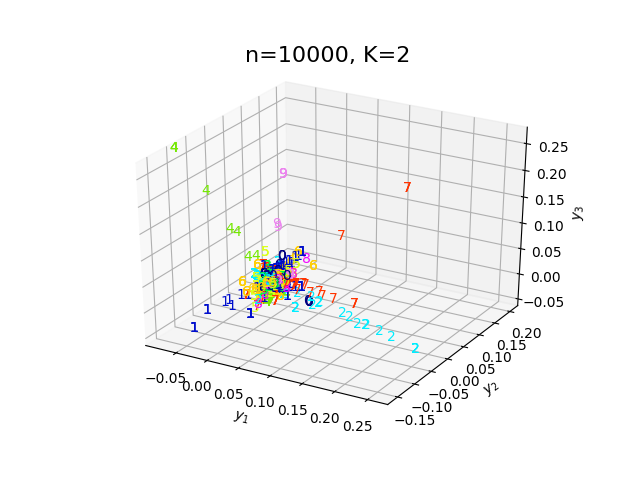
\includegraphics{3d_10000_2.png}}
    \end{subfigure}\\
    \begin{subfigure}[b]{0.45\textwidth}
    	\resizebox{\linewidth}{!}{
    	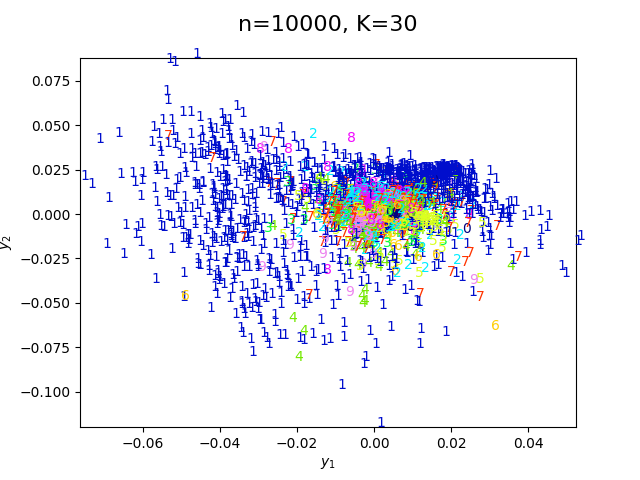
\includegraphics{2d_10000_30.png}}
    \end{subfigure}
    ~
    \begin{subfigure}[b]{0.45\textwidth}
    	\resizebox{\linewidth}{!}{
    	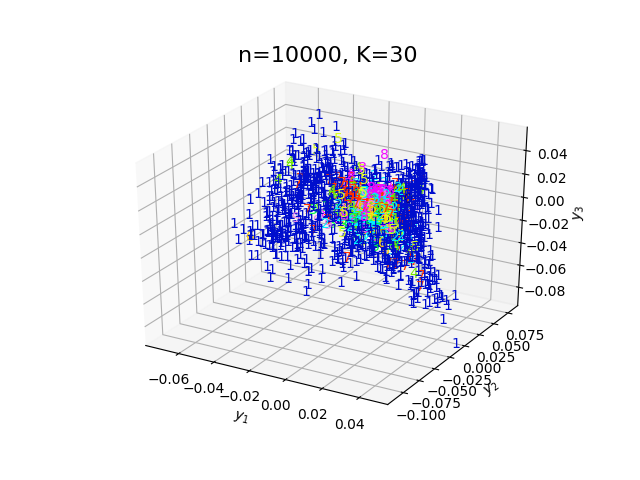
\includegraphics{3d_10000_30.png}}
    \end{subfigure}
    \caption{Visualizations of LLE in 2D and 3D for bad $K$.}
    \label{fig:plotBadK}
\end{figure}

\begin{figure}[H]
    \centering
    \begin{subfigure}[b]{0.45\textwidth}
    	\resizebox{\linewidth}{!}{
    	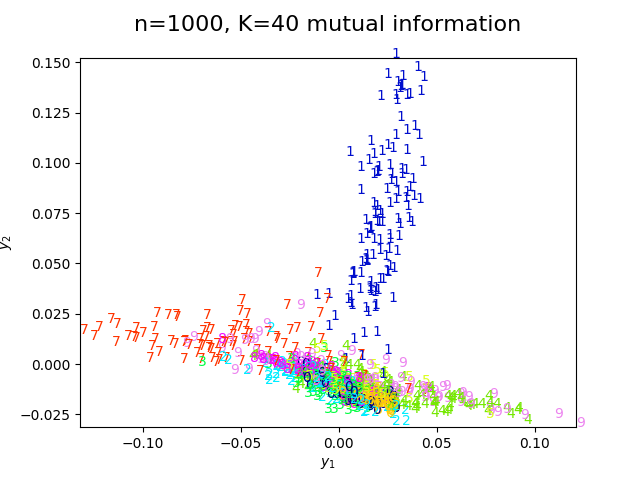
\includegraphics{mi_2d_1000_40.png}}
    \end{subfigure}
    ~
    \begin{subfigure}[b]{0.45\textwidth}
    	\resizebox{\linewidth}{!}{
    	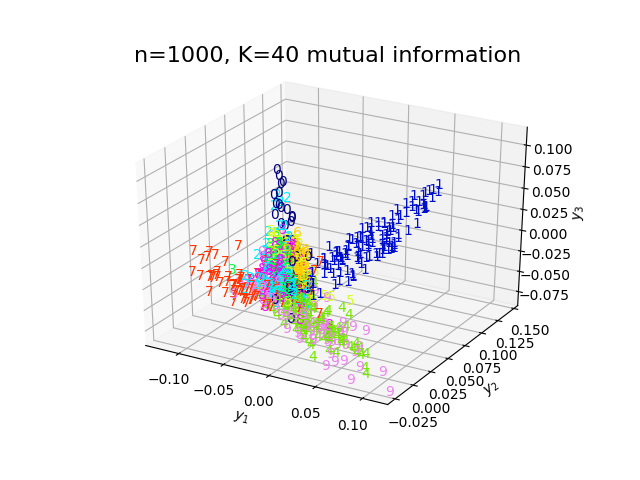
\includegraphics{mi_3d_1000_40.png}}
    \end{subfigure}
    \caption{Visualizations of LLE in 2D and 3D using mutual information to measure similarity for $K=40$.}
    \label{fig:plotMI40}
\end{figure}

\begin{figure}[H]
    \centering
    \begin{subfigure}[b]{0.45\textwidth}
    	\resizebox{\linewidth}{!}{
    	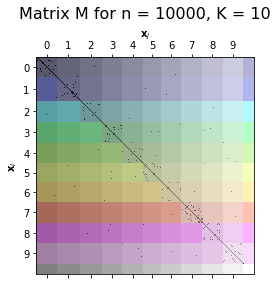
\includegraphics{M_10000.png}}
    \end{subfigure}
    \caption{Structure of matrix M.}
    \label{fig:M10k}
\end{figure}


\vspace{10pt}
\problemAnswer{ % Answer
\hmwkGitBranch % defined in line 5
}
\end{homeworkProblem}
\clearpage

\end{document}

